\section{Фајлови у   \textit{Lustre} систему}
Традиционални UNIX фајл системи користе чворове, који садрже спискове редних бројева блокова
где се чувају подаци о  фајлу за дати чвор. Слично томе, за сваки фајл у   \textit{Lustre} систему фајлова,
један чвор постоји на MDT-у. Међутим, у   \textit{Lustre} систему чвор на MDT није показивач на блок података, већ показује на један или више објеката коју су у вези са фајловима(слика 1.2). Ови објекти су датотеке на OST и садрже податке.

\begin{figure}[h!]
  \centering
      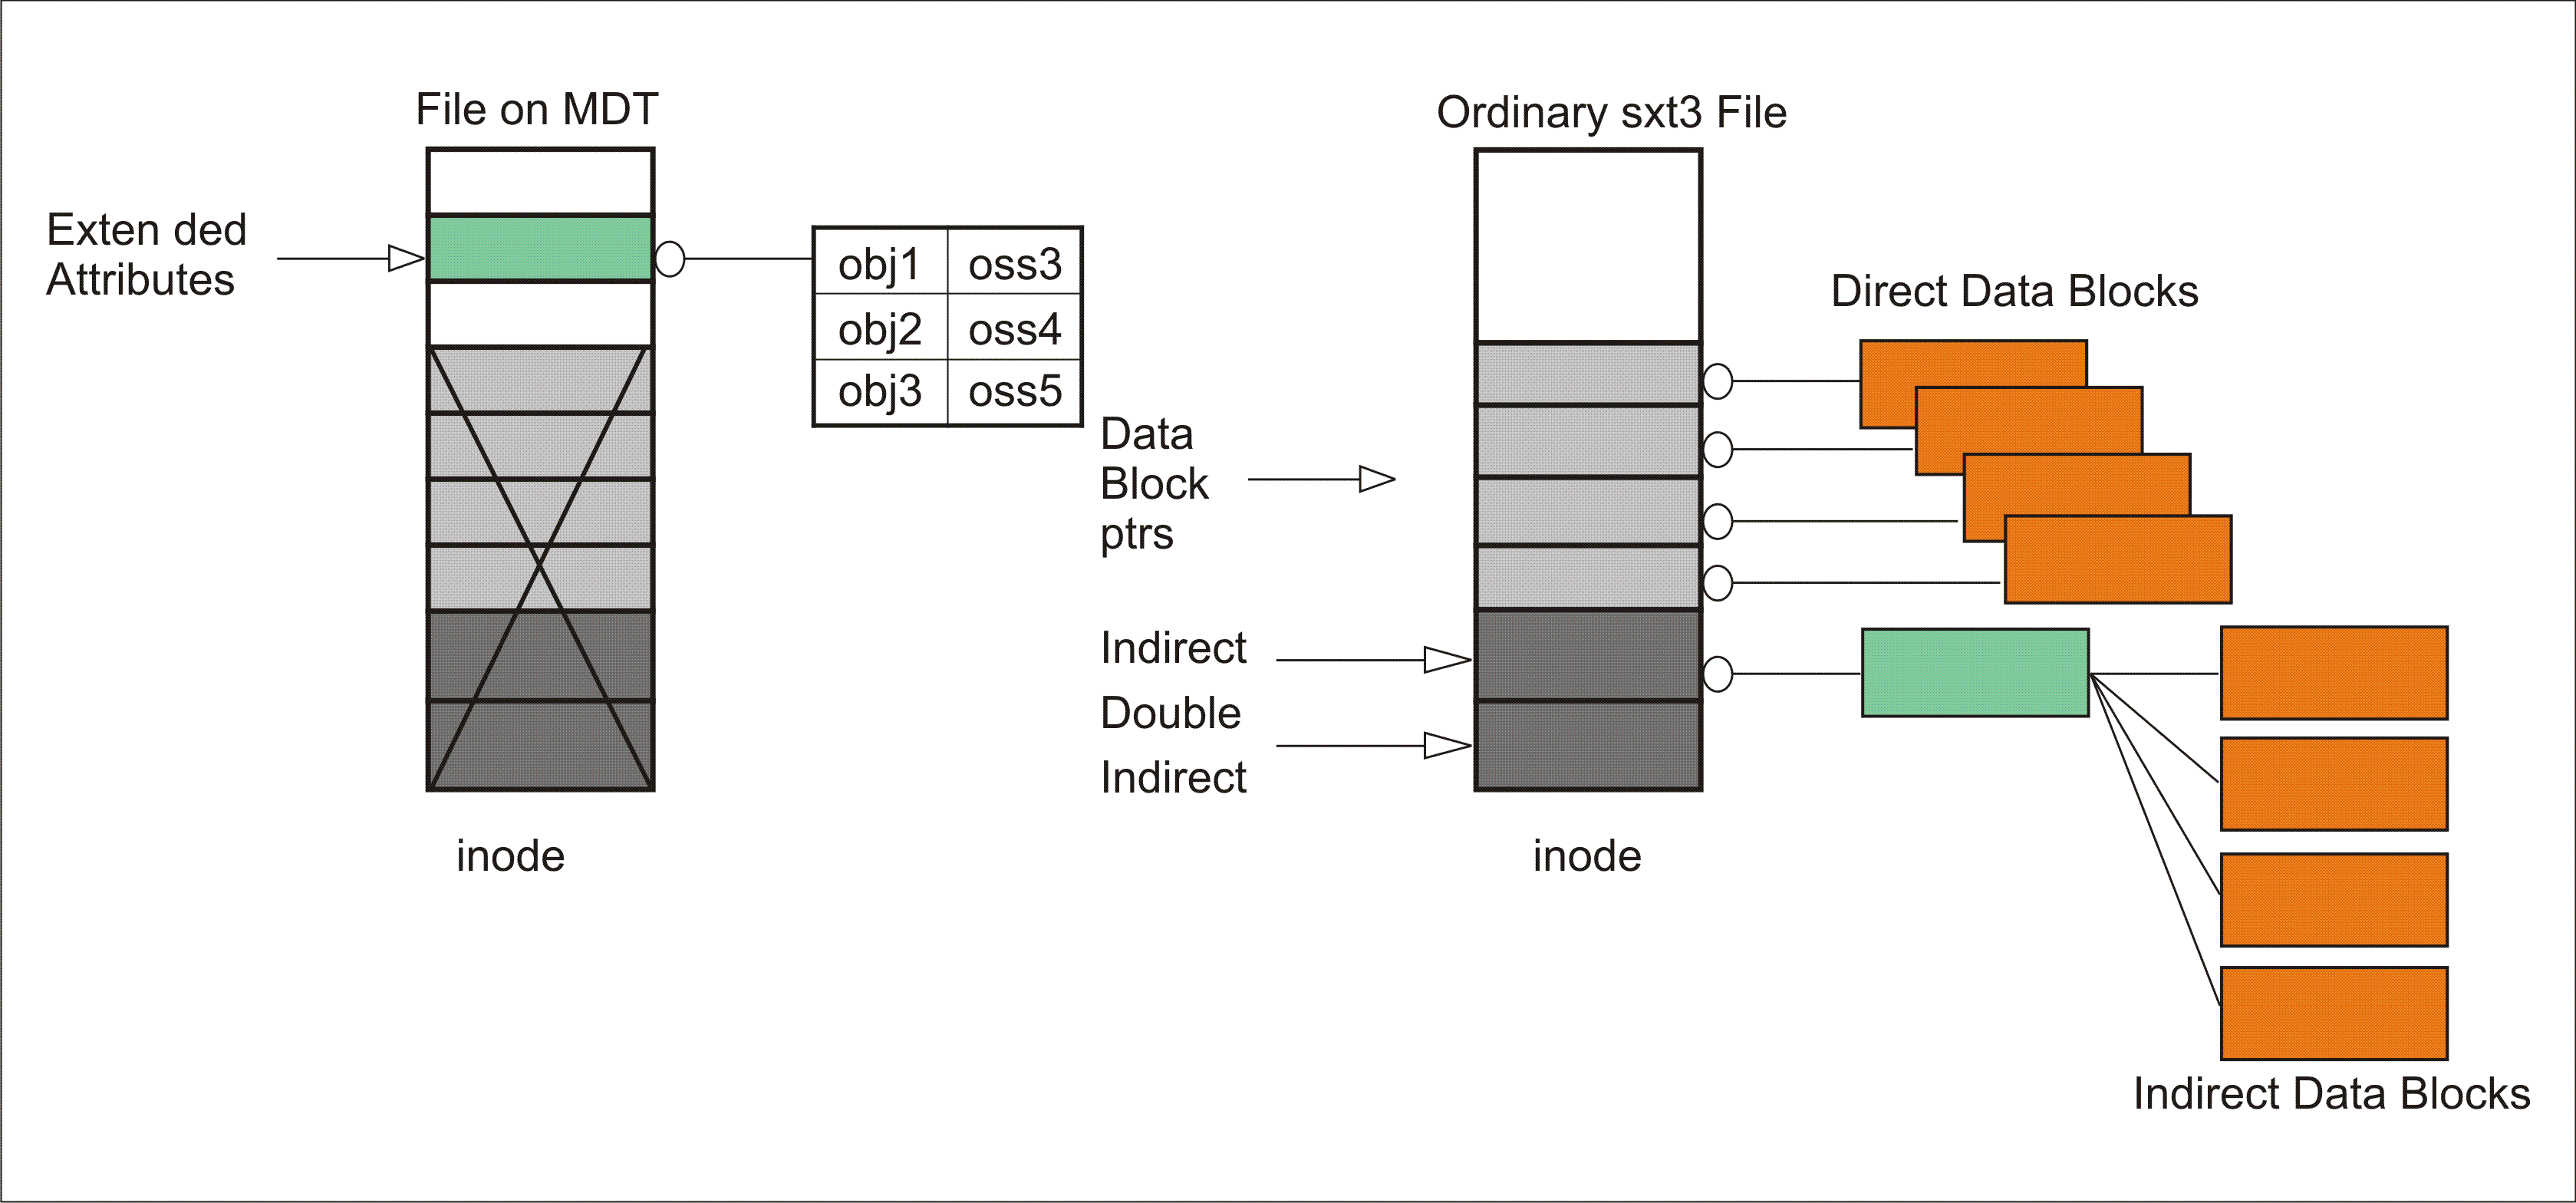
\includegraphics[width=1\textwidth]{slike/lustre_files.png}\\[1cm]
  \caption{Разлика измeђу MDS и ext3 чворова}
\end{figure}
\newpage

Уколико је само један објекат повезан са MDS чвор, тај објекат садржи све податке
у том систему. Када је више од једног објекта повезано, подаци у фајлу 
су подељени широм објекта. MDS зна распоред сваког фајла, број и локацију дела фајла. 
Клијенти добијају изглед фајла из MDS. Када клијент изврши  У/И операцију на делу фајла, 
фајл комуницира директно са релевантним OST-ом(слика 1.3). 

\begin{figure}[h!]
  \centering
      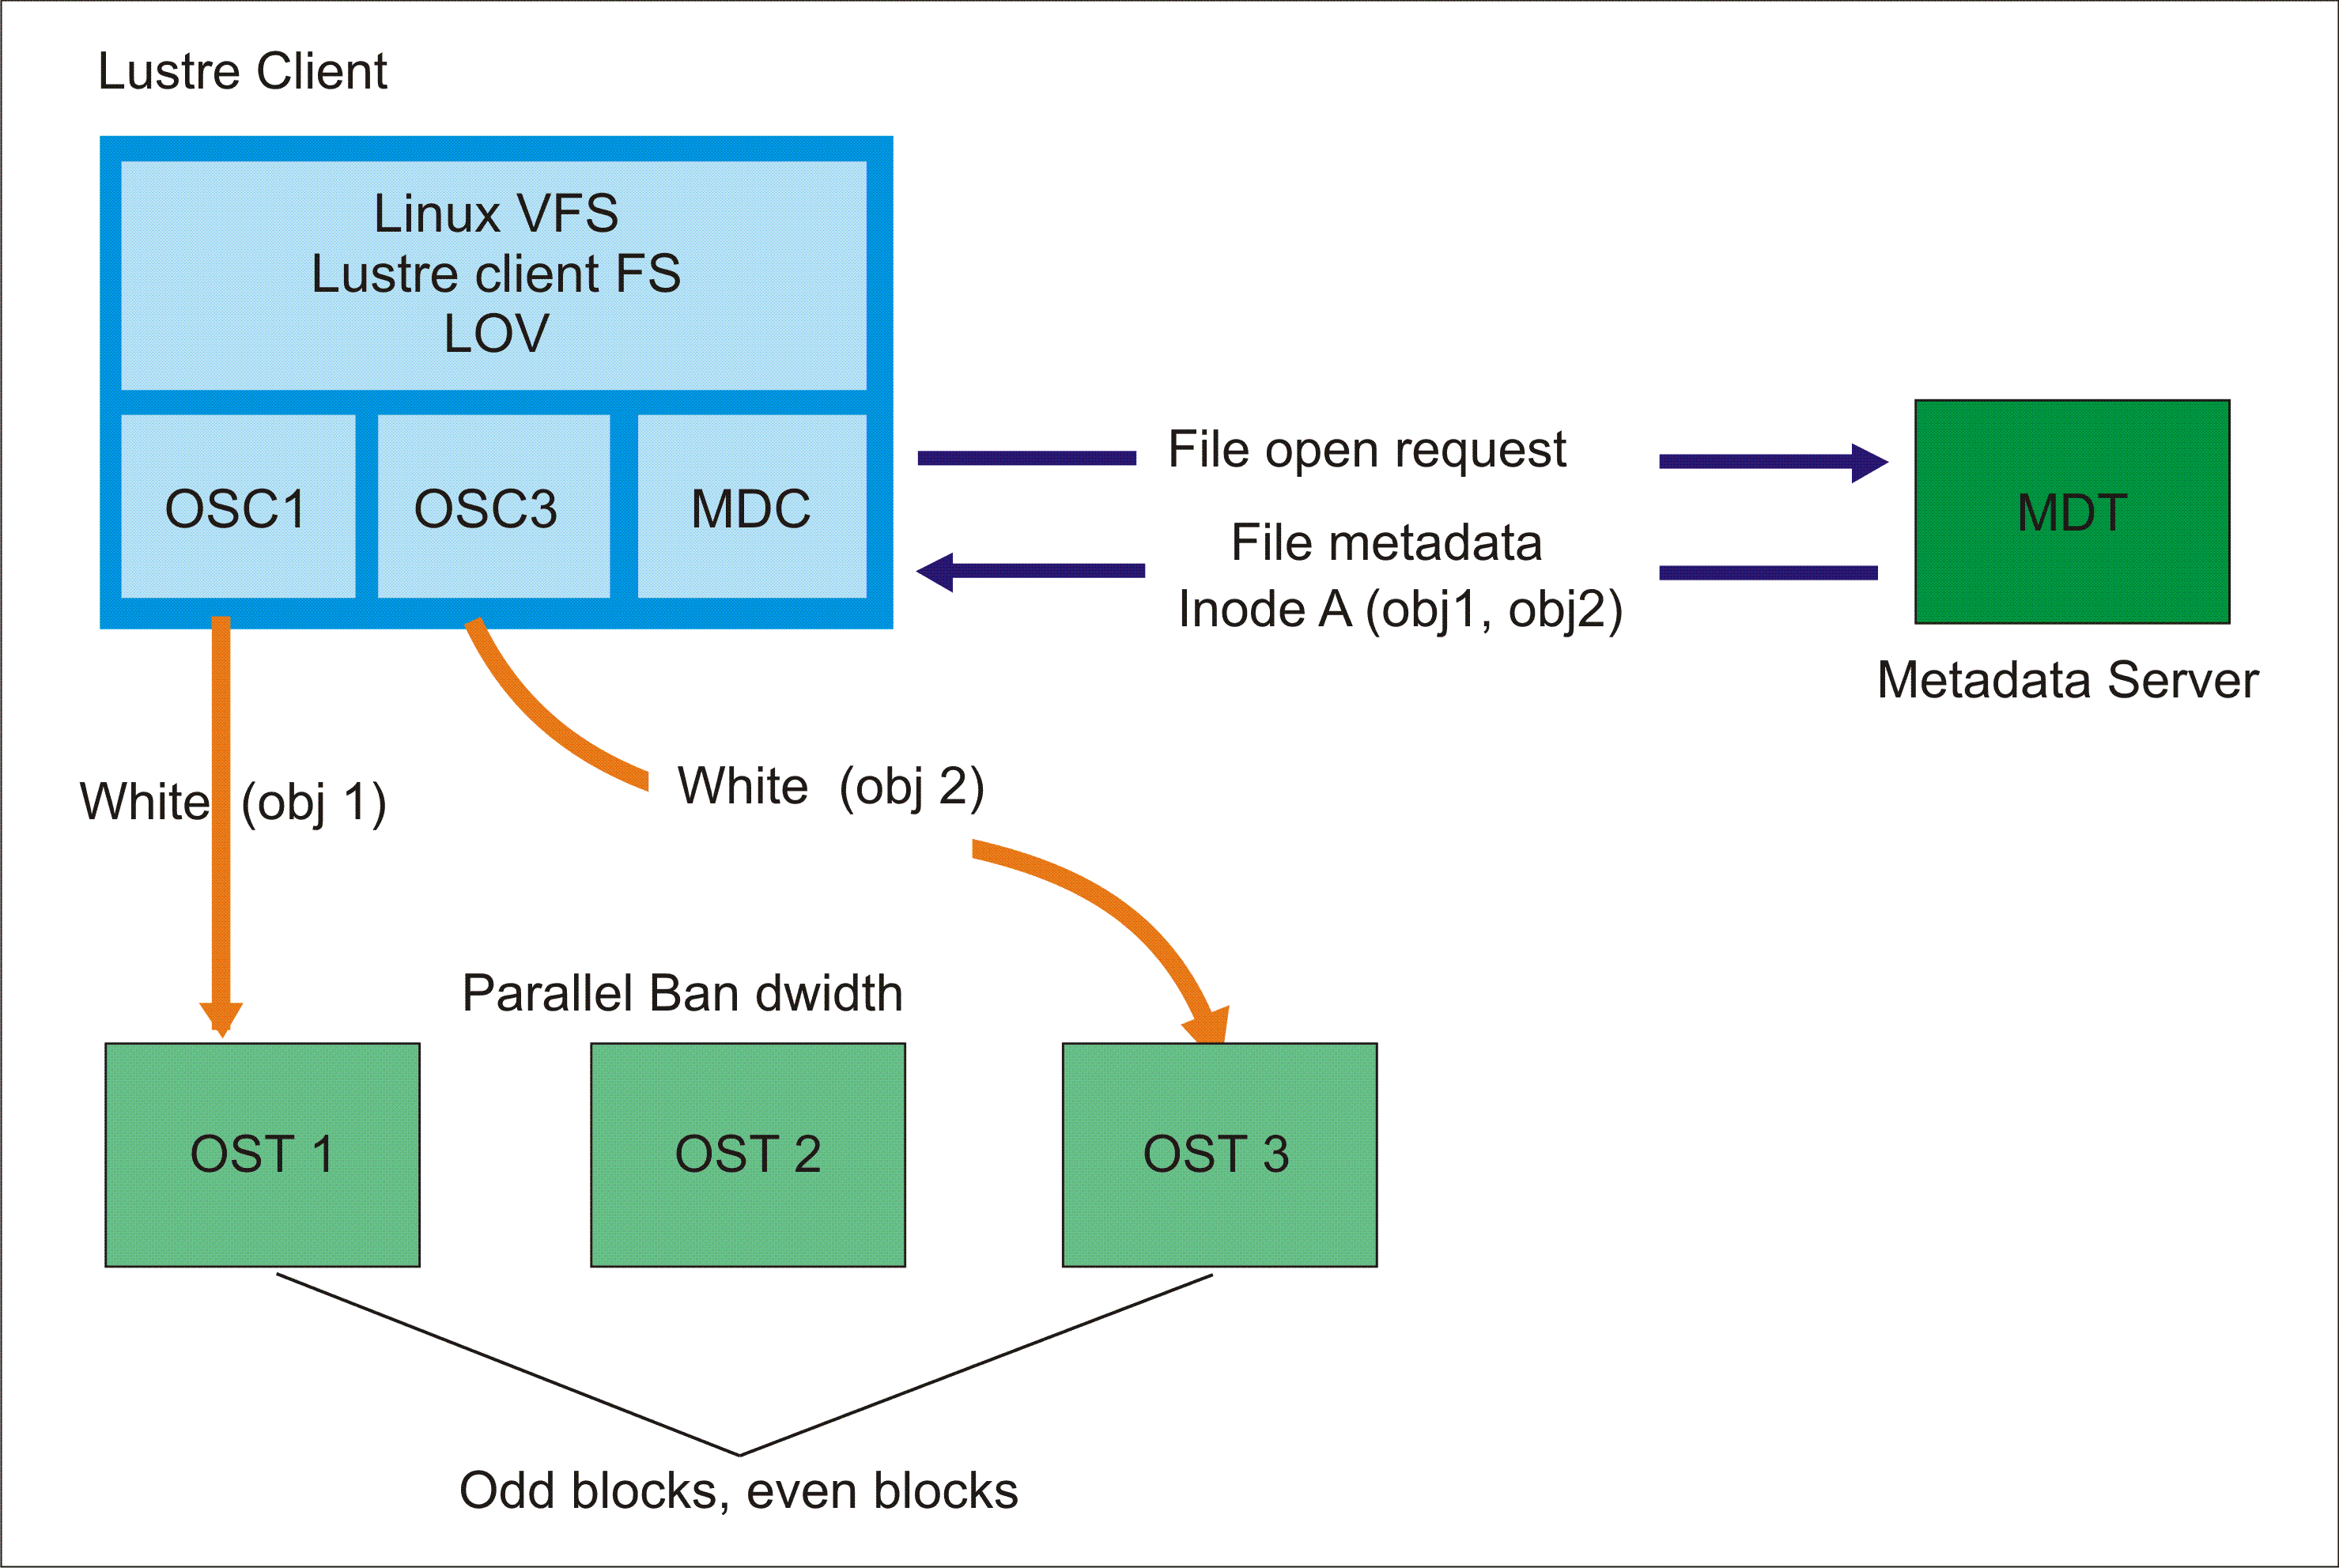
\includegraphics[width=1\textwidth]{slike/lustre_file_i_o.png}
  \caption{Lustre улазно/излазне операције}
\end{figure}

\subsection{Дељење фајлова у   \textit{Lustre}  систему}
Дељење фајлова омогућава да се делови фајлова чувају на различитим OST-има(слика 1.4). 
У RAID 0 нивоу подаци су подељени на већем броју објеката.

Број објеката се назива \textit{stripe\_count}. Сваки објекат садржи део податка. Када део податка који треба да се упише на одређени објекат прелази \textit{stripe\_count}, 
следећи део податка у датотеци се чува на следећем објекту. Дељење фајлова има  неколико предности. Једна је да максимална величина датотеке није 
ограничена величином једног OST. \textit{Lustre} може имати преко 160 подељених делова, и сваки део може да подржи максималну величину од 8TB. То доводи до максималне количине фајла од чак 1,48 PB. Још једна корист од дељења фајлова је та да је улазно/излазни пропусни опсег у једном фајлу 
збир улазно/излазних пропусних опсега за објекте од којих се фајл састоји. То у крајњем случају може бити проближно збиру пропусних опсега 160 сервера.


\begin{figure}[h!]
  \centering
      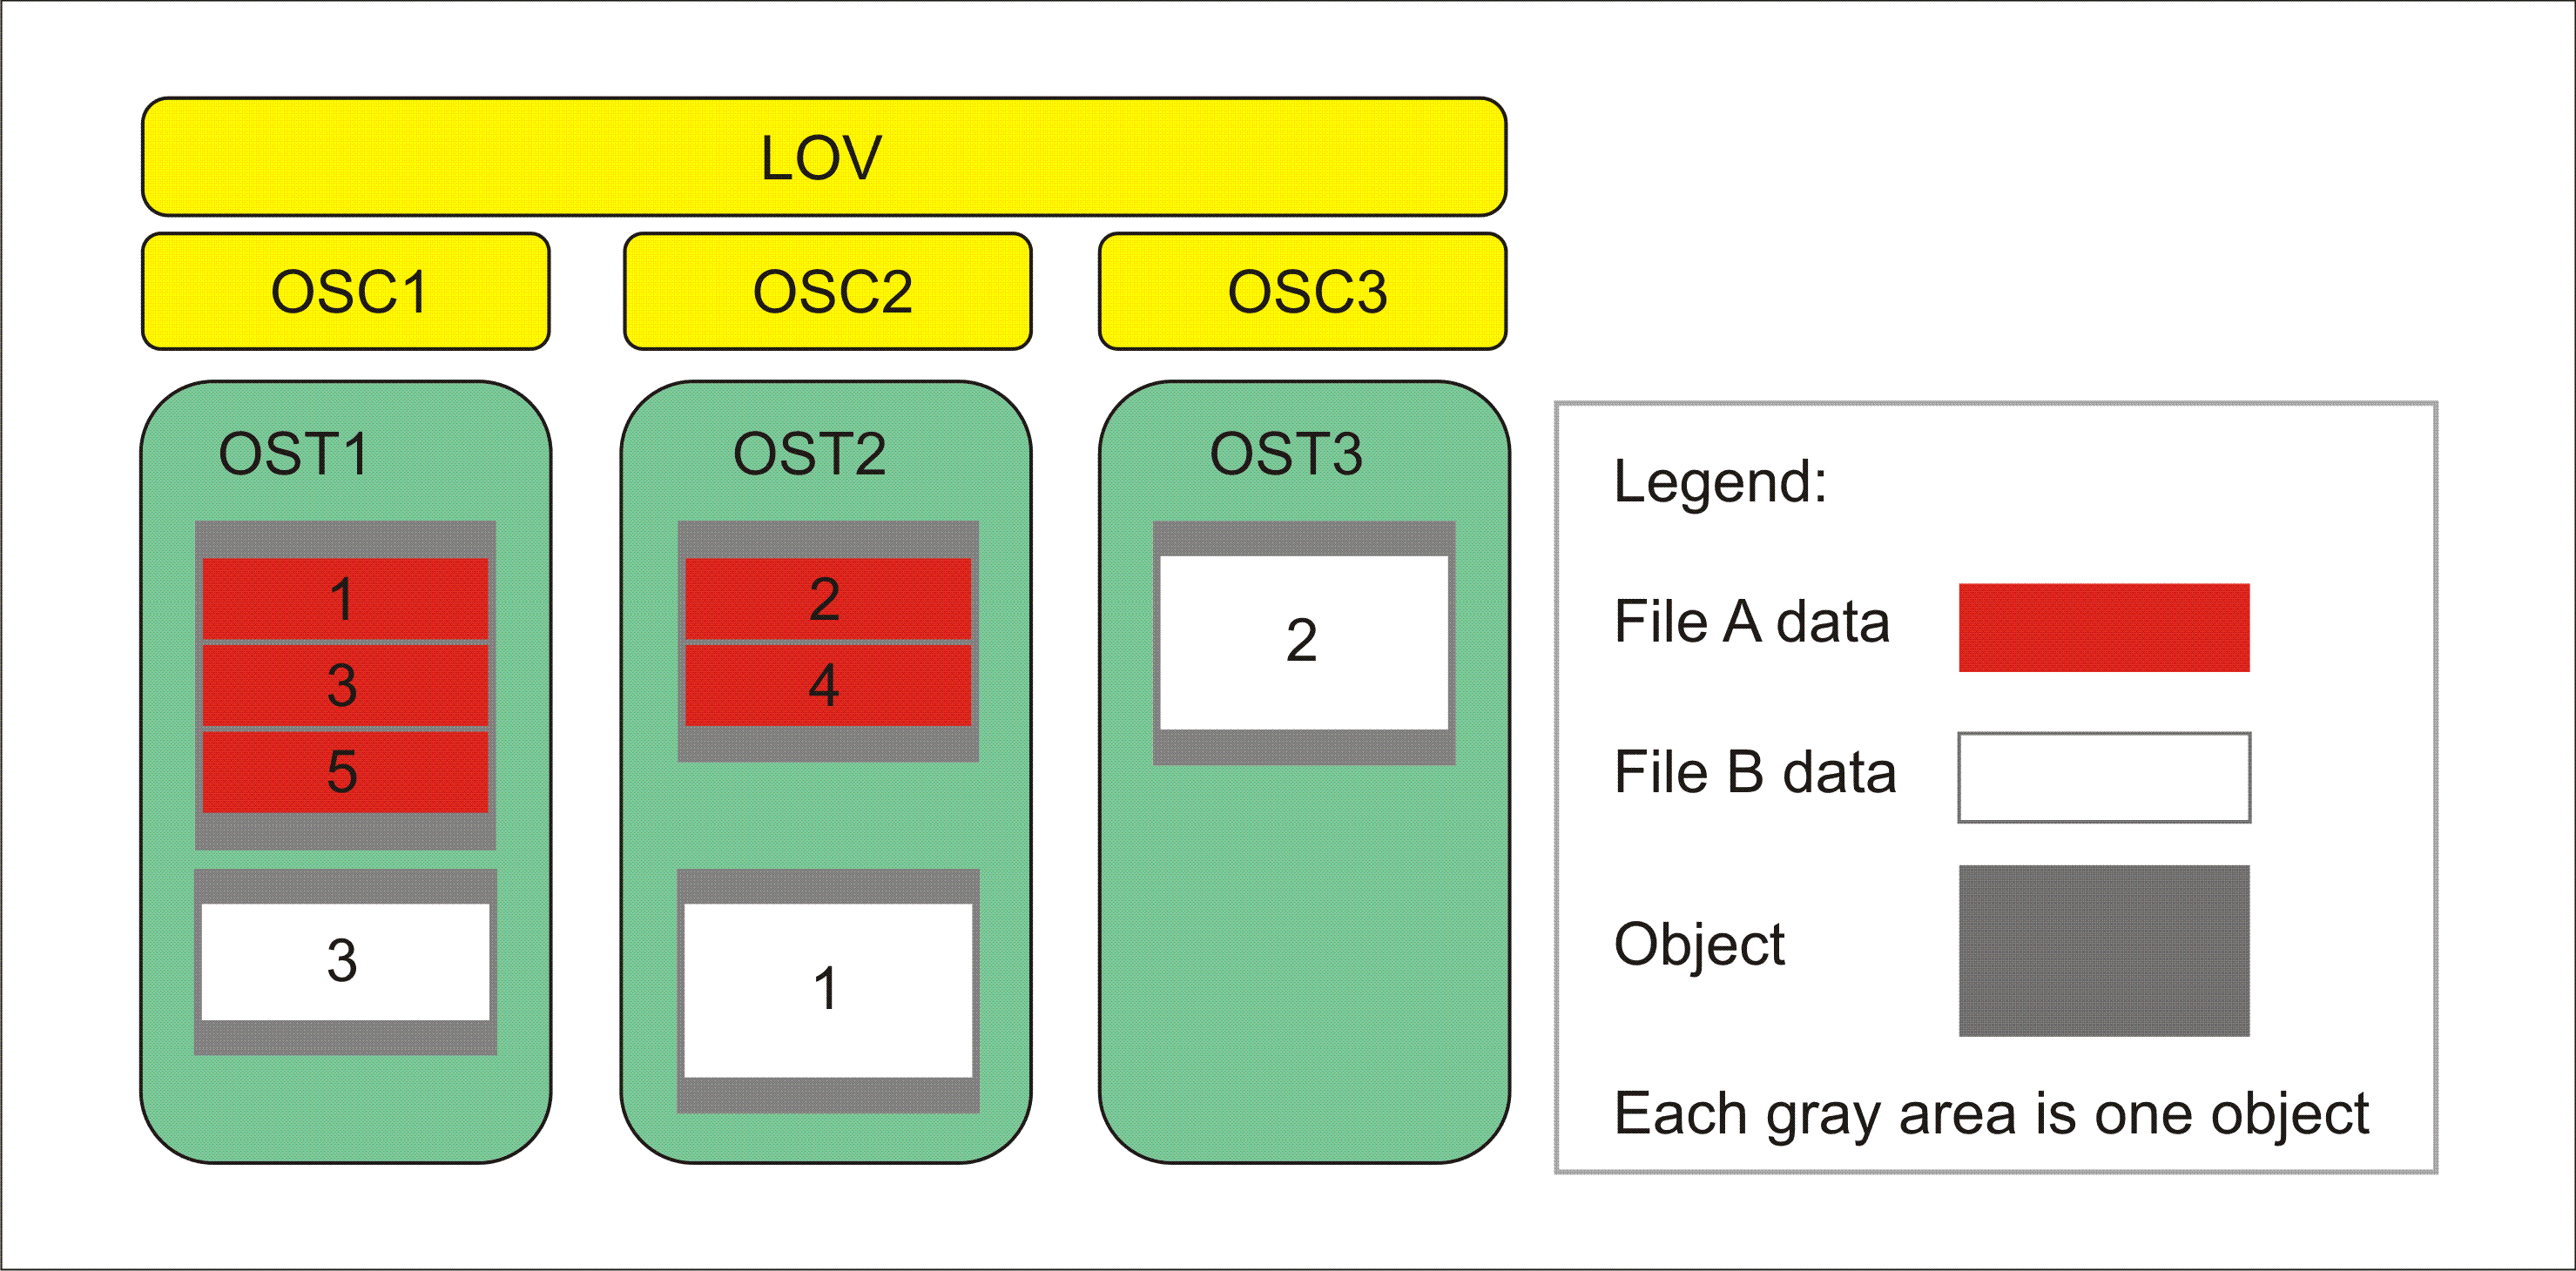
\includegraphics[width=1\textwidth]{slike/lustre_striping.png}
  \caption{Дељење фајлова}
\end{figure}

\subsection{\textit{Lustre} складиштење}
Складиштење у серверима је подељено, опционо организовано помоћу \textit{Logical
volume management (LVM)} система и форматирано као фајл систем. Lustre OSS и MDS
читају, пишу и мењају податке у формату који захтевају ови фајл системи.

\subsubsection{OSS складиштење}
Сваки OSS може управљати са више циљева за складиштење објеката (ОSТ-има), по један за сваки \textit{volume};
Улазно/излазни саобраћај је  избалансиран између ОSS-а и ОSТ-а. ОSS такође  треба да уравнотежи
пропусни опсег мреже између система мреже и складиштења и да спречи појаву уских грла. У зависности од карактеристика хардвера сервера, ОSS обично служи између 2 и 25 ОSТ-а, при чему је капацитет сваког од њих до 8 TB.

\subsubsection{MDS складиштење}
За MDS, складиштење мора бити везано за \textit{Lustre} метаподатке, за које је потребно 1-2 \% капацитета фајл система. Приступ подацима за MDS складиштење се разликује од приступа подацима за ОSS складиштења. 

\textit{Metadata} приступ подразумева рад са више захтева и читање-писање мале количине података, док улазно/излазни приступ подразумева пренос великих количина података. Велики проток података за MDS није превише битан, па се зато препоручује да се користе врсте складишта поппут FC или SAS дискова, који обезбеђују малу потражњу података. Са ниским нивоима улазно/излазних операција, RAID 5/6 није оптималан, док RAID 0+1 даје много боље резултате. \textit{Lustre} користи и \zn journaling" фајл система. За MDS се понекад могу добити и до 20 \%  бољи резултати уколико се  \zn journaling" фајл систем постави на различите дискове. Поред тога, MDS захтева велику снагу процесора и препоручује се барем четири процесорска језгра за оптималне перформансе.



